
\noindent\begin{minipage}{\textwidth}
    \begin{table}[H]
        \centering
        \caption{Hiperparâmetros e Resultados do Melhor Modelo - vit\_v8\_AB\_opt\_aug}
        \vspace{0.2cm}
        \resizebox{\textwidth}{!}{%
            \begin{tabular}{ll | lrrr}
                \hline
                \multicolumn{2}{c|}{\textbf{Hiperparâmetros}} & \multicolumn{4}{c}{\textbf{Métricas por Classe}} \\ \hline
                \textbf{Parâmetro} & \textbf{Valor} & \textbf{Classe} & \textbf{Precisão} & \textbf{Recall} & \textbf{F1-Score} \\ \hline
    Agendador (\$T\_0\$) & 15 & 31.2 & 0.3298 & 0.5442 & 0.4107 \\ 
Agendador de LR & CosineAnnealingWarmRestarts & 31.3 & 0.2885 & 0.0743 & 0.1181 \\ 
Architecture & vit\_b\_16 & 31.4 & 0.2434 & 0.2190 & 0.2306 \\ 
Augmentation (Método) & None & 32.3 & 0.2711 & 0.4745 & 0.3451 \\ 
Batch Size & 32 & 32.4 & 0.1739 & 0.0690 & 0.0988 \\ 
Decaimento de Peso (WD) & 0.0488 & 33.3 & 0.2327 & 0.1917 & 0.2102 \\ 
Dropout & 0.1236 & 41.4 & 0.1667 & 0.0909 & 0.1176 \\ 
Função de Perda & CrossEntropyLoss & 41.5 & 0.3000 & 0.3077 & 0.3038 \\ 
Hidden Units & 512 & 42.4 & 0.1333 & 0.0882 & 0.1062 \\ 
Label Smoothing & 0.0788 & 44.4 & 0.0000 & 0.0000 & 0.0000 \\ 
\cline{3-6} 
Otimizador & AdamW & \textbf{Média (Macro)} & 0.2139 & 0.2060 & 0.1941 \\ 
Taxa de Aprendizado (LR) & 5.24e-05 & \textbf{MCC} & \multicolumn{3}{c}{0.1436} \\ 
Unfreeze Layers & 3 &  & & &  \\ 
            \hline
            \end{tabular}%
        }
    \end{table}

    \begin{figure}[H]
        \centering
        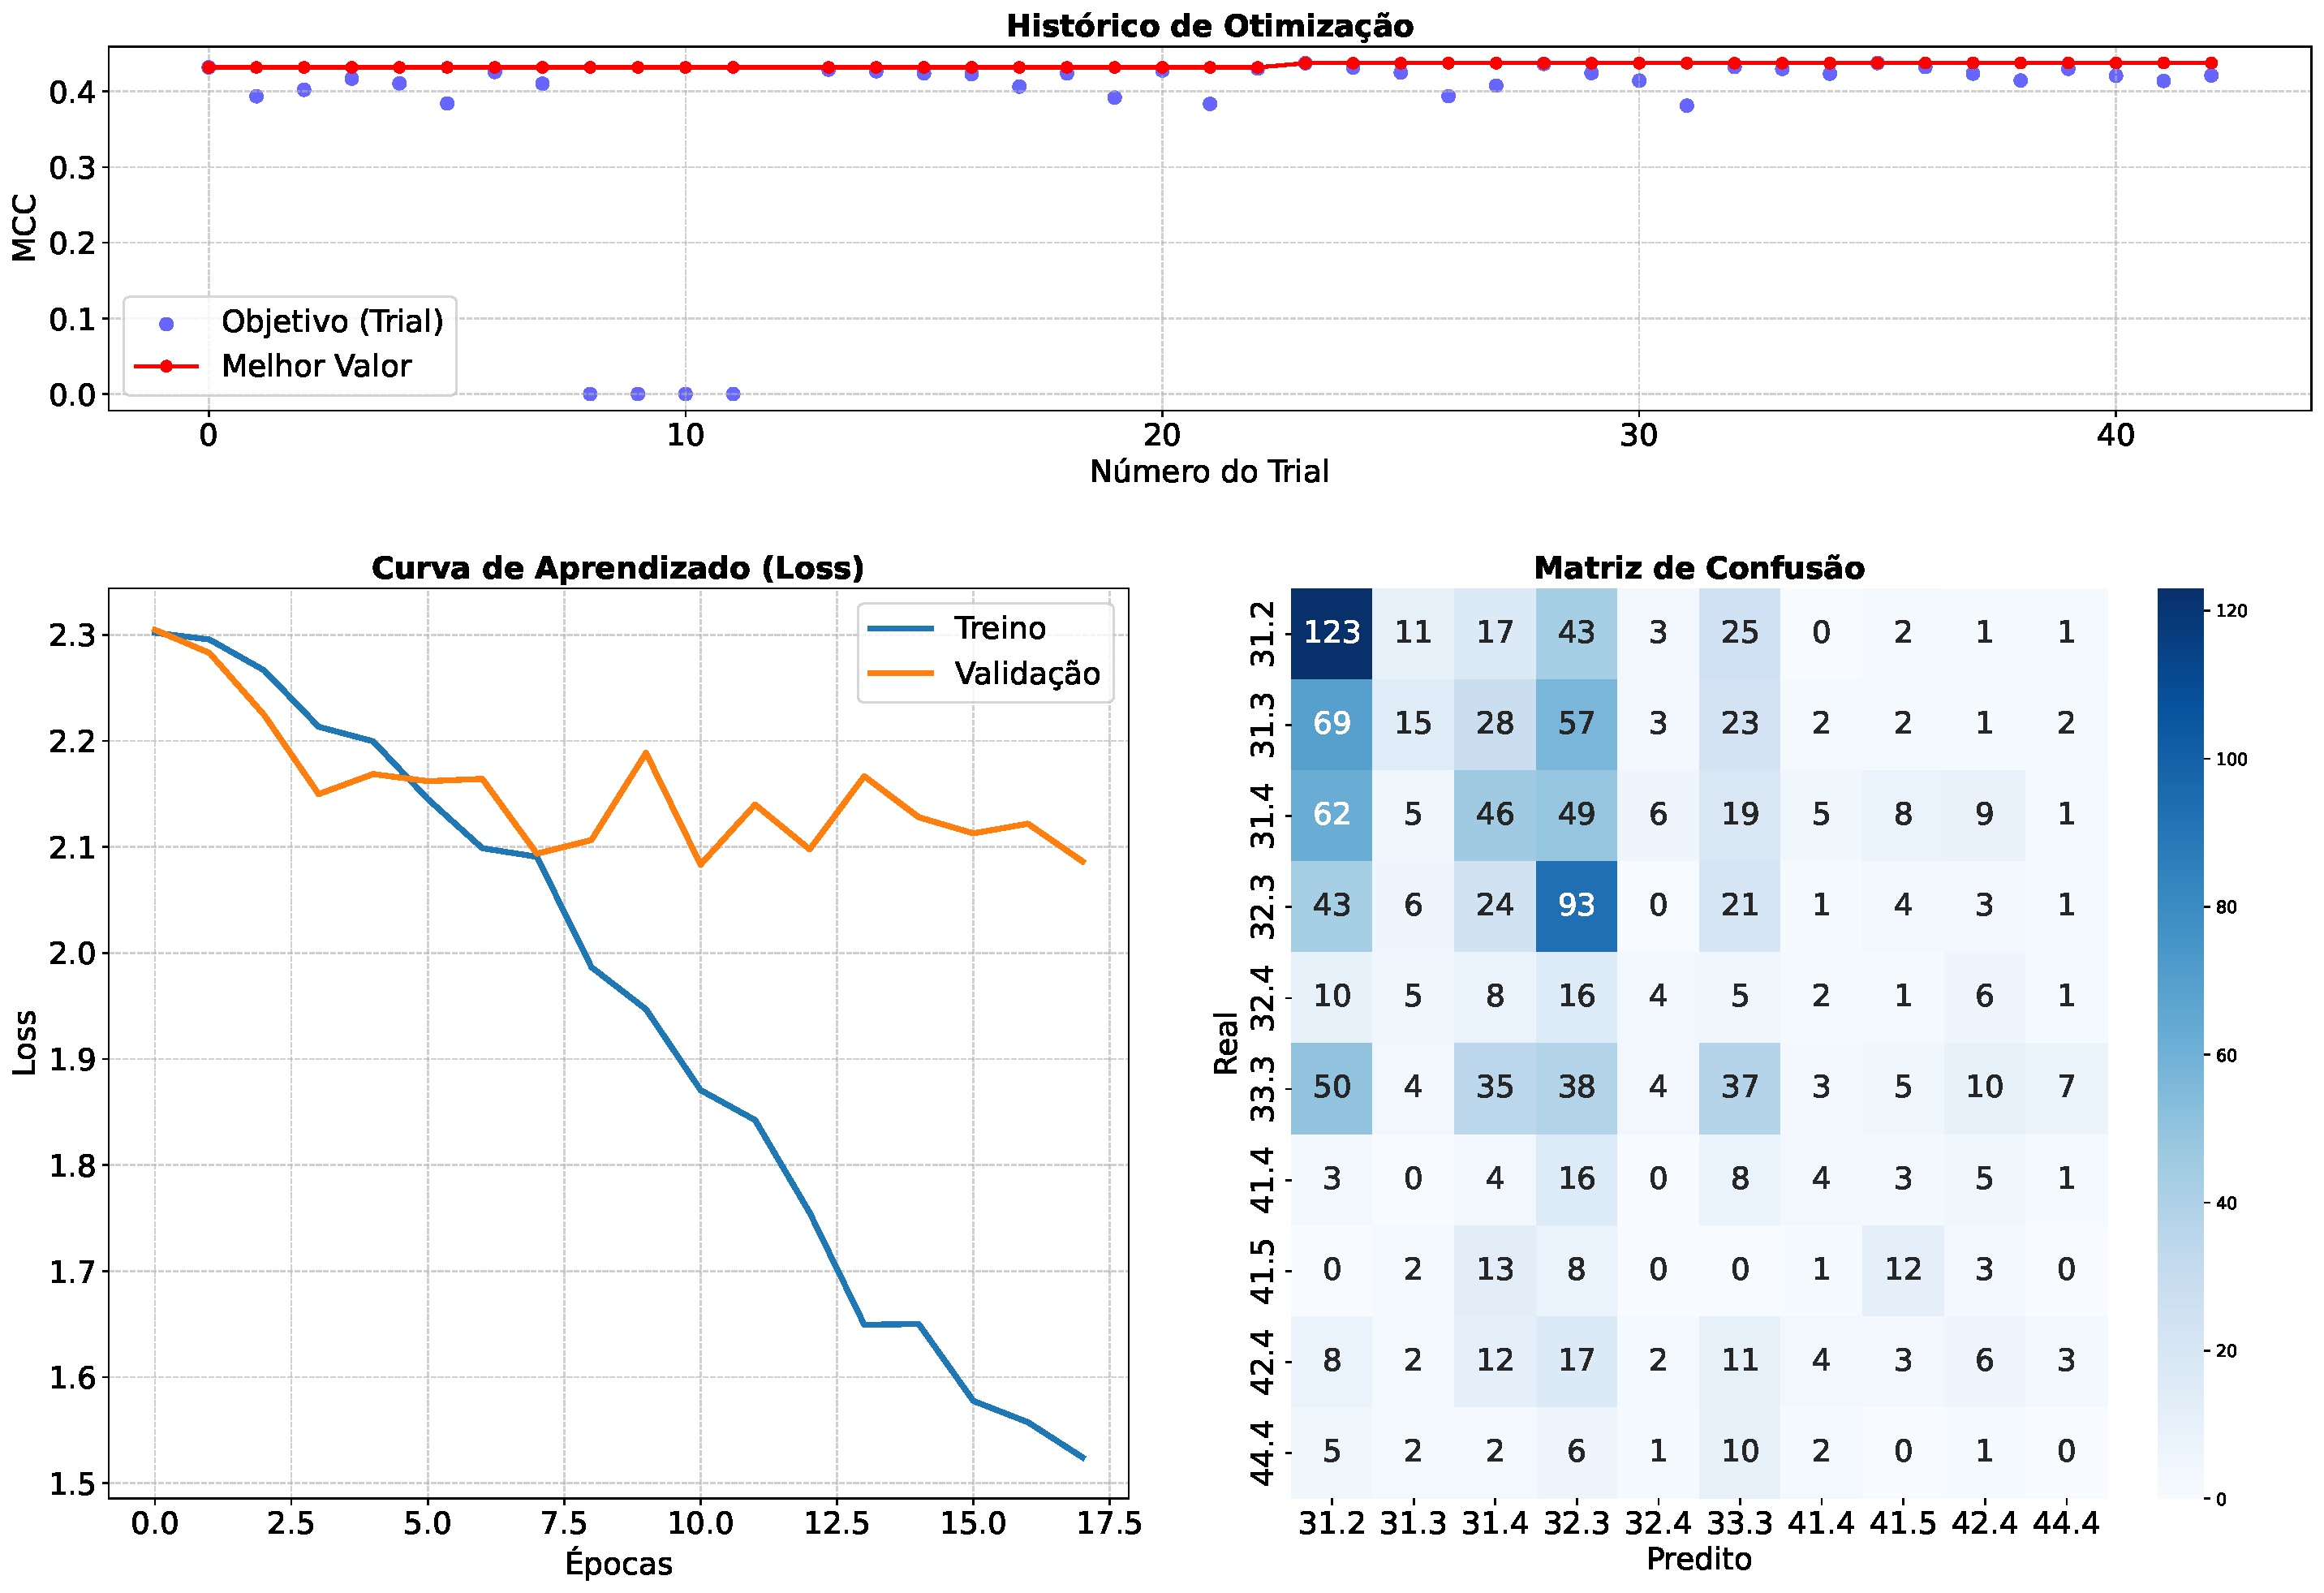
\includegraphics[width=0.85\textwidth]{tex/appendix/experiments/vit_v8_AB_opt_aug/dashboard_consolidado.pdf}
        \caption{Histórico de Otimização, Curvas de Aprendizado e Matriz de Confusão - vit\_v8\_AB\_opt\_aug}
    \end{figure}
\end{minipage}
\clearpage
